\documentclass[
%draft%     uncomment to activate draft mode (see preamble/proofs)
]{article}   

% preamble -- do not rearrange order of \includes
%\include{classoptions}
%\include{pagesize}
%\include{packages}
%\include{encoding}         
%\include{fonts}
%\include{ToC}
%\include{contributor}
%\include{copyright}
%\include{bibtex}
%\include{environments}
%\include{sectionoptions}
%\include{headerfooter}
%\include{footnoteformat}
%\include{codesnipets}
%\include{proofs}

\usepackage{tikz}
\usepackage{graphicx}
\usepackage[export]{adjustbox}
\usepackage{caption}
\usepackage{amssymb}
\usepackage{float}
\usepackage{subfig}
\usepackage{placeins}
\usepackage{listings}
\lstset{
  basicstyle=\ttfamily,
  mathescape
}
%\usepackage{minted}
\usetikzlibrary{shapes}
\usetikzlibrary {positioning}
\usetikzlibrary{chains}
\usetikzlibrary{fit}

\usepackage{geometry}
\usepackage{array}
\usepackage{hyperref}
\hypersetup{
    colorlinks=true,
    linkcolor=magenta,
    filecolor=cyan,      
    urlcolor=blue,
}
\graphicspath{ {./images/} }

% define issue details
\title{Compiler Optimization Notes}
\newcommand\thejournalsubtitle{Notes compiled for the Compiler Optimization Course}
\newcommand\thevolume{}
\newcommand\theseason{February}
\newcommand\theyear{2021}
\newcommand\theissue{\thejournal \ \thevolume \ (\theyear)} 
\newcommand\generaleditor{}
\newcommand\associateeditor{}
\sloppy
\newcommand\thewebsite{https://iitd.github.io/col729}

\begin{document}
\sloppy                         % preferences more space between words over overrunning margins
\lefthyphenmin=3                % suppresses hyphenation after only 1 or 2 characters
                                % NB: You will need to repeat \lefthyphenmin in the text if you use \selectlanguage
%\include{editorialboard}
%\include{titlepage}
%\include{colofon}
\pagenumbering{roman}           
%\tableofcontents  
\thispagestyle{empty}

\maketitle

% \include{essays/preface}
\pagenumbering{arabic}
%\part{COL729 Lecture Modules and Discussions}
\input{../module68}
\input{../module69} 
\input{../module70}
\input{../module71} 
\input{../module72}
\input{../module73} 
\input{../module74}
\input{../module75} 
\input{../module76}
\input{../module77} 
\input{../module78} 
\input{../module79}
\input{../module80}
\input{../feb19discussion}
\input{../module81} 
\input{../module82}
\input{../module83} 
\input{../module84}
\input{../feb26discussion}
\input{../module85} 
\input{../module86}
\input{../module87} 
\input{../module88}
\input{../module89}
\input{../module90}
\input{../module91} 
\input{../module92}
\input{../module93} 
\input{../module94}
\input{../module95} 
\input{../module96}
\input{../module97} 
\input{../module98}
\input{../module99} 
\input{../module100}
\section{Partial Redundancy Elimination}
\begin{flushright}
\textit{Notes by Akshin Singh}
\end{flushright}

A particularly good place to optimize is in loops. Since loops can run for a million iterations, moving any computation from 
inside the loop to outside while maintaing correctness is a desirable optimization. Such kind of optimization is called loop invariant
code motion. 

\begin{figure}[h]
\centering
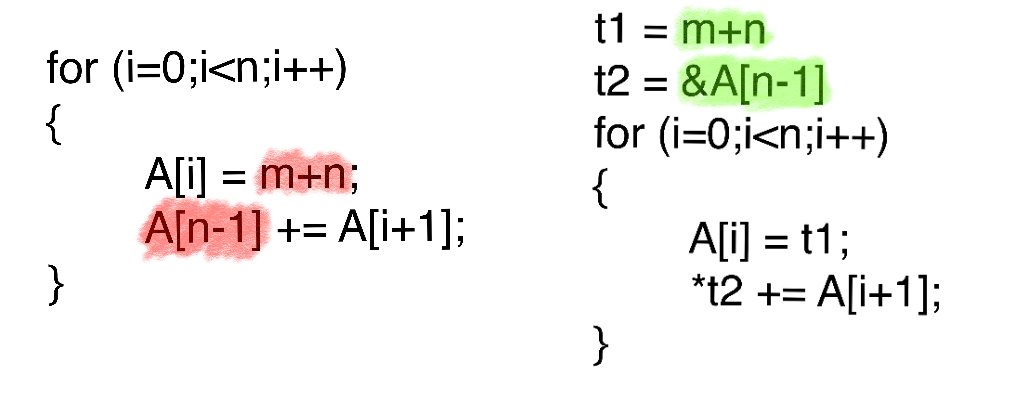
\includegraphics[scale = 0.5]{images/mod_105_fig1.png}
\caption{Loop invariant Code Motion Example}
\label {fig:mod_105_01}
\end{figure}

Let us explain with the help of an example. See the original code present in Figure \ref{fig:mod_105_01}. Since i is the loop variable,
that gets incremented every iteration, both \textbf{A[i]} and \textbf{A[i+1]} are dependent on the loop's progress. Hence these variables
are not invariant. However, the expression \textbf{m+n} and \textbf{A[n-1]} are both loop invariant. This is because both n and m hold their
values across iterations. We can therefore transform the code as shown.

Notice that since we have removed an addition as well as an address calculation (which is a multiply and add instruction), we have reduced
the number of instructions in the loop by two. Now if the loop runs a million times, we have saved a lot of work (typically on the order of 
two to three hunderd cycles). 

What happens if the loop does not run even once? Our transformed code will then have two extra instructions and we have inadvertently slowed
ourseleves by optimizing. This is the tradeoff that an optimizing compiler decides to make or not. 

\subsection{Partial Redundancy Elimination}

Let us take a deeper look into why we wanted to transform code in \ref{fig:mod_105_01}. Let us try to follow the control of the program.
We enter the program and then enter the loop. Inside the loop we calculate \textbf{m+n} and \textbf{A[n-1]} in the first iteration. 
Then, before the values of m and n are changed we subsequently calculated \textbf{m+n} and \textbf{A[n-1]} again in the next iteration. 

Keeping this in mind, let us define the problem of Partial Redundancy. If an expression is redundant (we will 
define redundancy in a while) on any path leading to it, it is said to be partially redundant. This is not the case in Common subexpression
elimination, where we can remove only those expressions which are completely redundant, i.e., redundant on all paths. 

\begin{figure}[h]
\centering
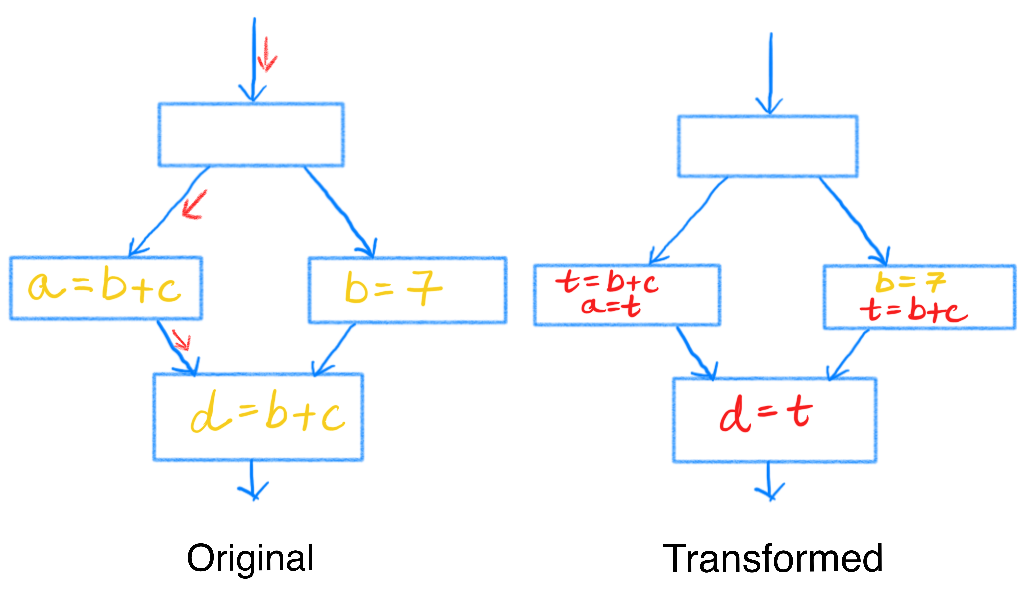
\includegraphics[scale = 0.5]{images/mod_105_fig2.png}
\caption{Partial Redundancy Elimination Example}
\label {fig:mod_105_02}
\end{figure}

A clearer example can be seen in Figure \ref{fig:mod_105_02}. Here \textbf{b+c} is redundant on the path from \textbf{a=b+c} and not on the 
other path. The transformed code has no redundancy. Partial Redundancy Elimination (or PRE for short) is the problem of placing computations (like \textbf{a=b+c}) such that no path recomputes
the same expression.

\begin {itemize}
\item Since PRE is a general optimization that does not need to work on only loops, PRE subsumes Loop invariant code motion. This is because
any computation that is loop invariant is redundant on the path that goes from the loop body back to the loop body.  

\begin{figure}[h]
\centering
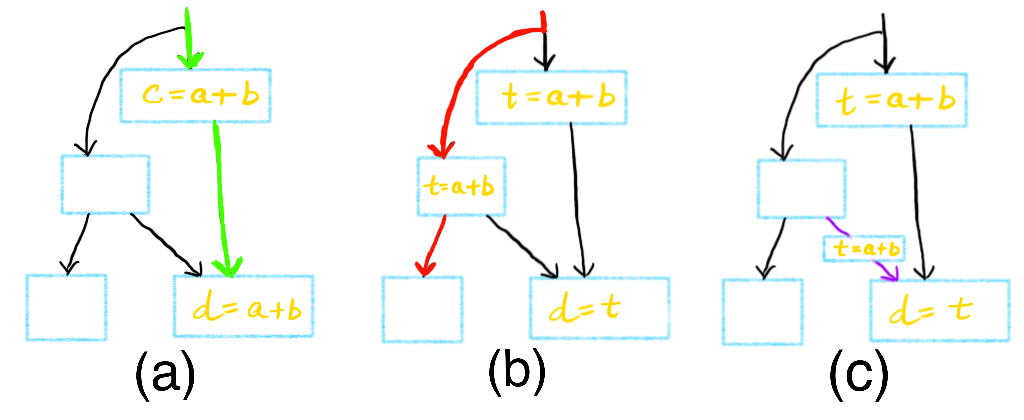
\includegraphics[scale = 0.3]{images/mod_105_fig3.png}
\caption{Redundancy Example}
\label {fig:mod_105_03}
\end{figure}

\item PRE may require addition of basic blocks. To understand this we need to define redundancy. Let us first take an example. Figure 
\ref{fig:mod_105_03}(a) has a redundancy on the green path. If the computation is moved as shown in \ref{fig:mod_105_03}(b), we have
a problem on the red path. The problem is that \textbf{a+b} is not needed anywhere on that path, and yet it is being computed. Naturally we
only want those computations to be present on a path that will be used eventually on that path. This leads us to define redundancy as 
any computation on a path that is either happening more than once if needed or at least once if not needed. To solve the problem, we need 
to add a basic block as shown in \ref{fig:mod_105_03}(c). Only then can we remove all partial redundancies.

Formally, the problem arised from the fact that we are hoisting computation across a \textbf{critical edge}. A critical edge is an edge
in the CFG where the source block has multiple successors and the desitination block has multiple predecessors. Hoisting across a critical
edge requires a new basic block since we may add redundancy on other paths. The pruple edge in \ref{fig:mod_105_03}(c) is the critical edge.

\item Even after adding basic blocks, there can be cases where we cannot elimate PRE until we decide to duplicate the code. See the 
Figure \ref{fig:mod_105_04}(a).

\begin{figure}[h]
\centering
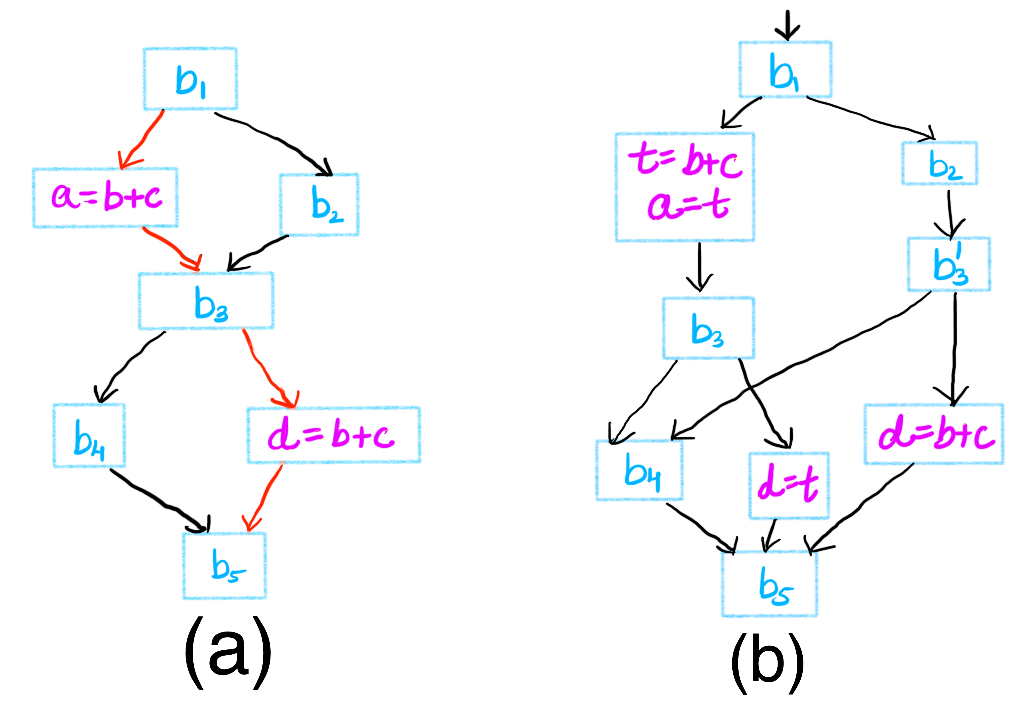
\includegraphics[scale = 0.3]{images/mod_105_fig4.png}
\caption{PRE Duplication Example}
\label {fig:mod_105_04}
\end{figure}

Here the expression \textbf{b+c} is redundant on the red path as shown. Here we need to duplicate the code as shown in 
Figure \ref{fig:mod_105_04}(b). Code duplication has caching effects. A larger code-size means a jump can be a jump to 
a far instruction which may incur a cache-miss which is not desirable, especially in today's out-of-order 6-8 wide issue processors. 
The penalty for i-cache miss can be very high. 
\end{itemize}
\section{Lazy Code Motion Problem}
\begin{flushright}
\textit{Notes by Akshin Singh}
\end{flushright}

As discussed in the previous module, the PRE problem has two components
\begin{enumerate}
\item All redundant computations of expressions that can be eliminated without duplication are eliminated.
\item The optimized program does not perform any extra computations that were not in the original program \textit{execution}.
\end{enumerate}

Lazy Code Motion (or LCM for short) adds another component to it.

\begin{enumerate}
  \setcounter{enumi}{2}
\item Expressions are computed at the late as possible (this is where the name \textbf{LAZY} comes from).
\end{enumerate}


\begin{figure}[h]
\centering
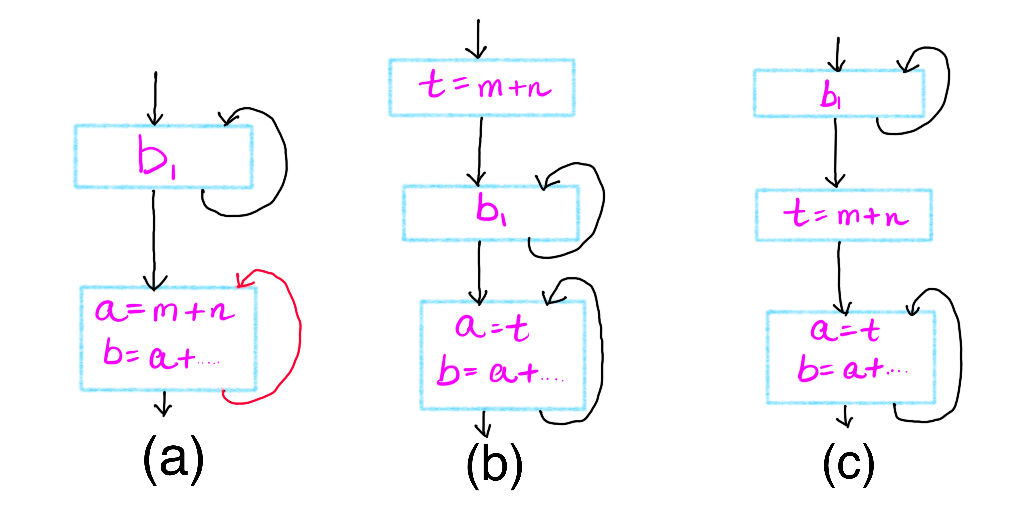
\includegraphics[scale = 0.5]{images/mod_106_fig1.png}
\caption{Lazy Code Motion example}
\label {fig:mod_106_01}
\end{figure}

Let us understand this with the help of an example. In Figure \ref{fig:mod_106_01}(a), we see that \textbf{m+n} is redundant on the red path,i.e., the loop's back edge. We will formally define what a back edge means in a later module. For now, the back edge means the edge that takes the execution from the loop's body back to its body.

PRE allows \ref{fig:mod_106_01}(b) but LCM does not. \textbf{WHY?} For PRE, components 1 and 2 are satisified in \ref{fig:mod_106_01}(b). For LCM component 3 is not satisfied. We can see this from the fact that the loop consisting of b1 needs to hold the value of \textbf{m+n} even though it does not need it. LCM component 3 is satisfied in \ref{fig:mod_106_01}(c).

Notice how \ref{fig:mod_106_01}(c) is a solution for both LCM and PRE whereas \ref{fig:mod_106_01}(b) is a solution for PRE but not LCM. This example suggests that $PRE \subset LCM$. In other words, LCM subsumes PRE. This is expected since PRE shares both its rules with LCM, but LCM has extra conditions as well.

\subsection{Full vs Partial Redundancy}

As eluded to in the last module, an expression is fully redundant at a program point if it is redundant on all paths to that program point. If an expressions is redundant on some but not all paths, then that expression is partially redundant.

Another way to frame what PRE does is the following: \textit{Can we place additional copies of an expression e which is partially redundant at program point p, such that it becomes fully redundant at p?} A fully redundant expression can be easily eliminated using common subexpression elimination.


\textbf{For more examples see the lecture module 106 on YouTube}.




%\include{../module101} 
%\include{../module102}
%\include{../module103} 
%\include{../module104}
%\section{Partial Redundancy Elimination}
\begin{flushright}
\textit{Notes by Akshin Singh}
\end{flushright}

A particularly good place to optimize is in loops. Since loops can run for a million iterations, moving any computation from 
inside the loop to outside while maintaing correctness is a desirable optimization. Such kind of optimization is called loop invariant
code motion. 

\begin{figure}[h]
\centering
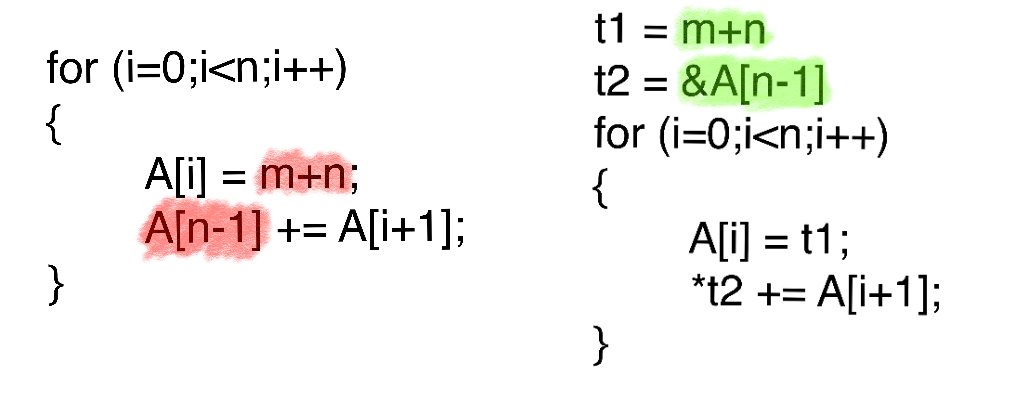
\includegraphics[scale = 0.5]{images/mod_105_fig1.png}
\caption{Loop invariant Code Motion Example}
\label {fig:mod_105_01}
\end{figure}

Let us explain with the help of an example. See the original code present in Figure \ref{fig:mod_105_01}. Since i is the loop variable,
that gets incremented every iteration, both \textbf{A[i]} and \textbf{A[i+1]} are dependent on the loop's progress. Hence these variables
are not invariant. However, the expression \textbf{m+n} and \textbf{A[n-1]} are both loop invariant. This is because both n and m hold their
values across iterations. We can therefore transform the code as shown.

Notice that since we have removed an addition as well as an address calculation (which is a multiply and add instruction), we have reduced
the number of instructions in the loop by two. Now if the loop runs a million times, we have saved a lot of work (typically on the order of 
two to three hunderd cycles). 

What happens if the loop does not run even once? Our transformed code will then have two extra instructions and we have inadvertently slowed
ourseleves by optimizing. This is the tradeoff that an optimizing compiler decides to make or not. 

\subsection{Partial Redundancy Elimination}

Let us take a deeper look into why we wanted to transform code in \ref{fig:mod_105_01}. Let us try to follow the control of the program.
We enter the program and then enter the loop. Inside the loop we calculate \textbf{m+n} and \textbf{A[n-1]} in the first iteration. 
Then, before the values of m and n are changed we subsequently calculated \textbf{m+n} and \textbf{A[n-1]} again in the next iteration. 

Keeping this in mind, let us define the problem of Partial Redundancy. If an expression is redundant (we will 
define redundancy in a while) on any path leading to it, it is said to be partially redundant. This is not the case in Common subexpression
elimination, where we can remove only those expressions which are completely redundant, i.e., redundant on all paths. 

\begin{figure}[h]
\centering
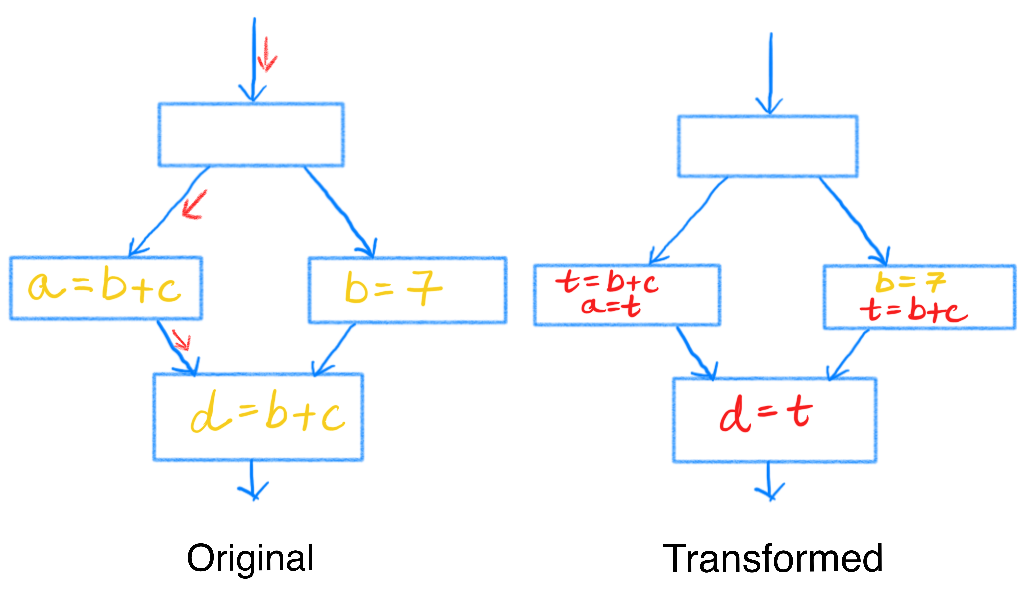
\includegraphics[scale = 0.5]{images/mod_105_fig2.png}
\caption{Partial Redundancy Elimination Example}
\label {fig:mod_105_02}
\end{figure}

A clearer example can be seen in Figure \ref{fig:mod_105_02}. Here \textbf{b+c} is redundant on the path from \textbf{a=b+c} and not on the 
other path. The transformed code has no redundancy. Partial Redundancy Elimination (or PRE for short) is the problem of placing computations (like \textbf{a=b+c}) such that no path recomputes
the same expression.

\begin {itemize}
\item Since PRE is a general optimization that does not need to work on only loops, PRE subsumes Loop invariant code motion. This is because
any computation that is loop invariant is redundant on the path that goes from the loop body back to the loop body.  

\begin{figure}[h]
\centering
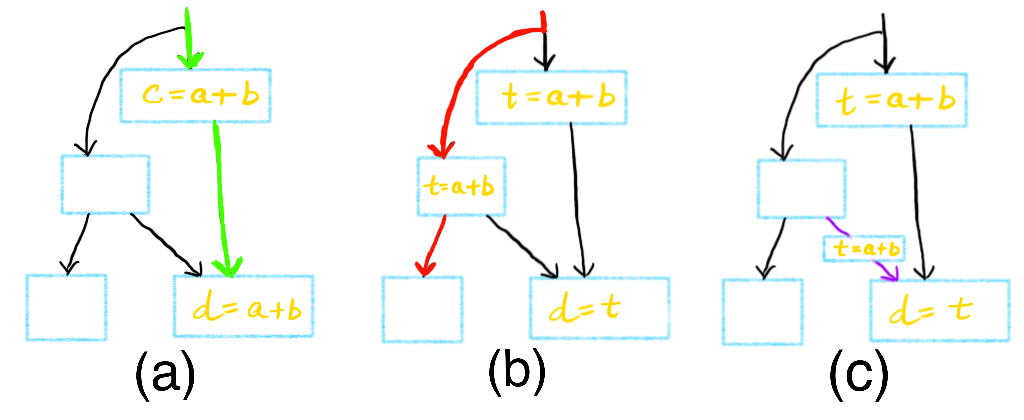
\includegraphics[scale = 0.3]{images/mod_105_fig3.png}
\caption{Redundancy Example}
\label {fig:mod_105_03}
\end{figure}

\item PRE may require addition of basic blocks. To understand this we need to define redundancy. Let us first take an example. Figure 
\ref{fig:mod_105_03}(a) has a redundancy on the green path. If the computation is moved as shown in \ref{fig:mod_105_03}(b), we have
a problem on the red path. The problem is that \textbf{a+b} is not needed anywhere on that path, and yet it is being computed. Naturally we
only want those computations to be present on a path that will be used eventually on that path. This leads us to define redundancy as 
any computation on a path that is either happening more than once if needed or at least once if not needed. To solve the problem, we need 
to add a basic block as shown in \ref{fig:mod_105_03}(c). Only then can we remove all partial redundancies.

Formally, the problem arised from the fact that we are hoisting computation across a \textbf{critical edge}. A critical edge is an edge
in the CFG where the source block has multiple successors and the desitination block has multiple predecessors. Hoisting across a critical
edge requires a new basic block since we may add redundancy on other paths. The pruple edge in \ref{fig:mod_105_03}(c) is the critical edge.

\item Even after adding basic blocks, there can be cases where we cannot elimate PRE until we decide to duplicate the code. See the 
Figure \ref{fig:mod_105_04}(a).

\begin{figure}[h]
\centering
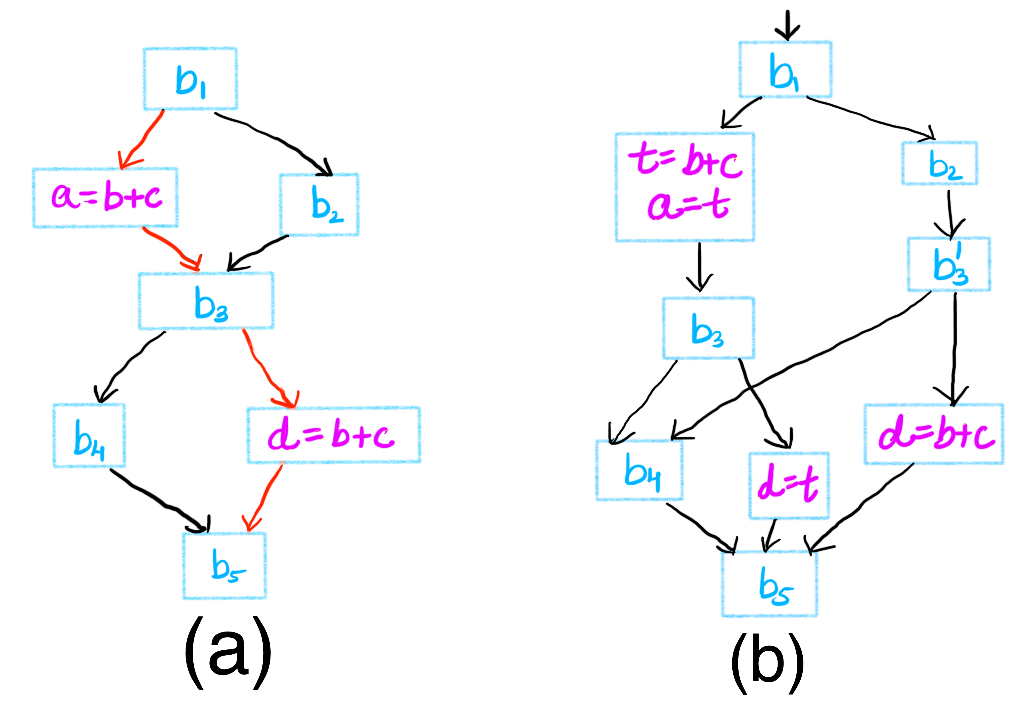
\includegraphics[scale = 0.3]{images/mod_105_fig4.png}
\caption{PRE Duplication Example}
\label {fig:mod_105_04}
\end{figure}

Here the expression \textbf{b+c} is redundant on the red path as shown. Here we need to duplicate the code as shown in 
Figure \ref{fig:mod_105_04}(b). Code duplication has caching effects. A larger code-size means a jump can be a jump to 
a far instruction which may incur a cache-miss which is not desirable, especially in today's out-of-order 6-8 wide issue processors. 
The penalty for i-cache miss can be very high. 
\end{itemize} 
%\section{Lazy Code Motion Problem}
\begin{flushright}
\textit{Notes by Akshin Singh}
\end{flushright}

As discussed in the previous module, the PRE problem has two components
\begin{enumerate}
\item All redundant computations of expressions that can be eliminated without duplication are eliminated.
\item The optimized program does not perform any extra computations that were not in the original program \textit{execution}.
\end{enumerate}

Lazy Code Motion (or LCM for short) adds another component to it.

\begin{enumerate}
  \setcounter{enumi}{2}
\item Expressions are computed at the late as possible (this is where the name \textbf{LAZY} comes from).
\end{enumerate}


\begin{figure}[h]
\centering
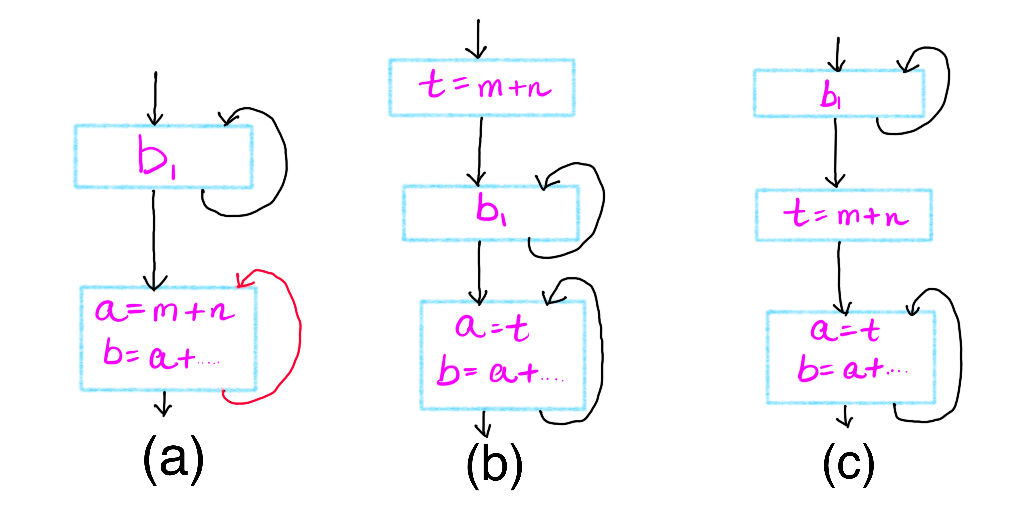
\includegraphics[scale = 0.5]{images/mod_106_fig1.png}
\caption{Lazy Code Motion example}
\label {fig:mod_106_01}
\end{figure}

Let us understand this with the help of an example. In Figure \ref{fig:mod_106_01}(a), we see that \textbf{m+n} is redundant on the red path,i.e., the loop's back edge. We will formally define what a back edge means in a later module. For now, the back edge means the edge that takes the execution from the loop's body back to its body.

PRE allows \ref{fig:mod_106_01}(b) but LCM does not. \textbf{WHY?} For PRE, components 1 and 2 are satisified in \ref{fig:mod_106_01}(b). For LCM component 3 is not satisfied. We can see this from the fact that the loop consisting of b1 needs to hold the value of \textbf{m+n} even though it does not need it. LCM component 3 is satisfied in \ref{fig:mod_106_01}(c).

Notice how \ref{fig:mod_106_01}(c) is a solution for both LCM and PRE whereas \ref{fig:mod_106_01}(b) is a solution for PRE but not LCM. This example suggests that $PRE \subset LCM$. In other words, LCM subsumes PRE. This is expected since PRE shares both its rules with LCM, but LCM has extra conditions as well.

\subsection{Full vs Partial Redundancy}

As eluded to in the last module, an expression is fully redundant at a program point if it is redundant on all paths to that program point. If an expressions is redundant on some but not all paths, then that expression is partially redundant.

Another way to frame what PRE does is the following: \textit{Can we place additional copies of an expression e which is partially redundant at program point p, such that it becomes fully redundant at p?} A fully redundant expression can be easily eliminated using common subexpression elimination.


\textbf{For more examples see the lecture module 106 on YouTube}.




%\include{../module107} 
%\include{../module108}
%\include{../module109} 
%\include{../module110}
%\include{../module111} 
%\include{../module112}
%\include{../module113} 
%\include{../module114}
%\include{../module115} 
%\include{../module116}
%\include{../module117} 
%\include{../module118}
%\include{../module119} 
\section{Computational Structure of a Region-Based DFA}
\FloatBarrier
\begin{flushright}
    \textit{Scribed by Arpit Saxena}
\end{flushright}

\begin{enumerate}
    \item {
        Identify transfer function of each region (and sub-region)

        \textbf{Bottom-up pass:}
        \begin{enumerate}
            \item Basic blocks transfer function derived from individual 
            statement's transfer functions 
            \item Loop body's transfer function from basic block's transfer 
            function
            \item Loop's from loop body's, \ldots
        \end{enumerate}
    }
    \item {
        Compute the dataflow values at each program point by using the summary
        transfer functions (for entire regions)

        \textbf{Top-down analysis}: Descend down the region hierarchy
        for internal points
    }

    
\end{enumerate}

\begin{figure}[H]
    \centering
    \subfloat[\label{fig:m120:ex1:a}] {{
        \tt
        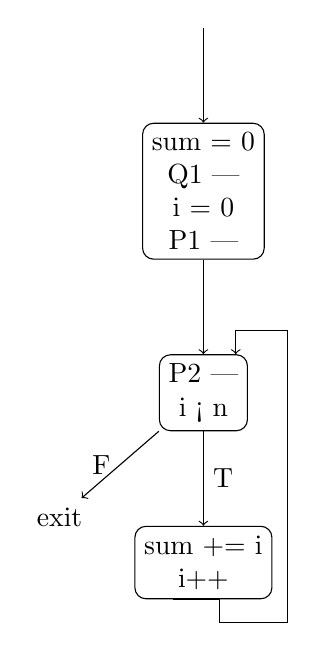
\begin{tikzpicture}[->,
            node distance = 12mm,
            start chain = going below,
            box/.style = {draw,rounded corners,fill=white,
                on chain,align=center},
            unbox/.style = {on chain,align=center},
            edge/.style = {midway}]
            \coordinate[on chain] (begin);
            \node[box] (b1) {
                sum = 0\\
                Q1 --- \\
                i = 0 \\
                P1 ---
            };
            \node[box] (b2) {
                P2 --- \\
                i < n
            };
            \node[unbox,below left=of b2] (b3) {exit};
            \node[box,below=of b2] (b4) {sum += i \\ i++};
            \path[]
                (begin) edge (b1)
                (b1) edge (b2)
                (b2) edge node[edge, left] {F} (b3)
                    edge node[edge, right] {T} (b4);
            \draw (b4.230) -| ++(0.6,-0.3) -| ([xshift=5mm]b2.east) |-
            ([yshift=3mm]b2.50) -- (b2.50);
        \end{tikzpicture}
    }}
    \subfloat[\label{fig:m120:ex1:b}] {{
        \tt
        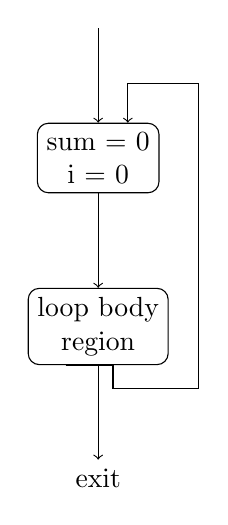
\begin{tikzpicture}[->,
            node distance = 12mm,
            start chain = going below,
            box/.style = {draw,rounded corners,fill=white,
                on chain,align=center},
            unbox/.style = {on chain,align=center},
            edge/.style = {midway}]
            \coordinate[on chain] (begin);
            \node[box](b1) {sum = 0 \\ i = 0};
            \node[box](b2) {loop body \\ region};
            \node[unbox](b3) {exit};
            \path[]
                (begin) edge (b1)
                (b1) edge (b2)
                (b2) edge (b3);
            \draw (b2.230) -| ++(0.6,-0.3) -| ([xshift=5mm]b1.east) |-
            ([yshift=5mm]b1.50) -- (b1.50);
            
        \end{tikzpicture}
    }}
    \subfloat[\label{fig:m120:ex1:c}] {{
        \tt
        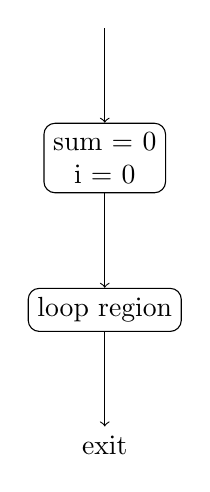
\begin{tikzpicture}[->,
            node distance = 12mm,
            start chain = going below,
            box/.style = {draw,rounded corners,fill=white,
                on chain,align=center},
            unbox/.style = {on chain,align=center},
            edge/.style = {midway}]
            \coordinate[on chain] (begin);
            \node[box](b1) {sum = 0 \\ i = 0};
            \node[box](b2) {loop region};
            \node[unbox](b3) {exit};
            \path[]
                (begin) edge (b1)
                (b1) edge (b2)
                (b2) edge (b3);
        \end{tikzpicture}
    }}
    \subfloat[\label{fig:m120:ex1:d}] {{
        \tt
        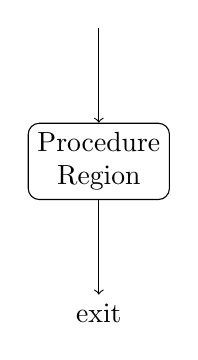
\begin{tikzpicture}[->,
            node distance = 12mm,
            start chain = going below,
            box/.style = {draw,rounded corners,fill=white,
                on chain,align=center},
            unbox/.style = {on chain,align=center},
            edge/.style = {midway}]
            \coordinate[on chain] (begin);
            \node[box](b1) {Procedure \\ Region};
            \node[unbox](exit) {exit};
            \path[]
                (begin) edge (b1)
                (b1) edge (exit);
        \end{tikzpicture}
    }}
    \caption{A Region Hierarchy\\ Note that P1, P2, \ldots\ are program points}
    \label{fig:m120:ex1}
\end{figure}

In figure \autoref{fig:m120:ex1:b}, the loop body's transfer function
would be:

{
    \centering
    \tt
    f\textsubscript{b}(m) = m' \\
    m'(i) = m(i) + 1 \\
    m'(sum) = m(sum) + m(i) \\
}

Based on f\textsubscript{b}, we'll try to create a summary transfer
function for the entire loop.

In figure \autoref{fig:m120:ex1:c}, the loop's transfer function would be

{
    \tt
    \centering
    m\textsuperscript{l} = f\textsubscript{l}(m) \\
    m\textsuperscript{l}(i) = max(m(i), n) \\
    m\textsuperscript{l}(sum) = m(sum) + $\sum_{j=m(i)}^{n-1} j$ \\
}

Note that if initially $i \geq n$, then the loop is not even entered, which
is the reason for having max in the second equation.

All iterations of the loop have been summarised as a single transfer function
f\textsubscript{l}, and it is a sophisticated symbolic analysis which may not
be possible for every loop. In that case, we have a fallback option of just
executing a basic DFA.

For figure \autoref{fig:m120:ex1:d}, we use the fact that we know at start of loop
region that \texttt{m(i) = 0, m(sum) = 0} and get the following transfer
function

{
    \tt
    \centering
    m\textsuperscript{p} = f\textsubscript{p}(m) \\
    m\textsuperscript{p}(i) = n \\
    m\textsuperscript{p}(sum) = n * (n - 1) / 2 \\
}

Note that the transfer function doesn't need to be a closed form function. It
only needs to be a computable (terminating) function.
E.g.: Trivial solutions based on fixed point (terminating because the lattices
have finite height).

Suppose we wanted to compute value at P1 (refer to \autoref{fig:m120:ex1}).

In top-down fashion, we start from the procedure region. If we needed Q1,
then f\textsubscript{1} (which transfer function for the first basic block
in figure \autoref{fig:m120:ex1:c}) would only give summary of the basic block.
So, we'll apply transfer function of \texttt{sum = 0}.

In general, at every level of the hierarchy: Compute the DFA values on that level
of the hierarchy and we'll get boundary values of next-level regions. If we're
interested in an internal point of a region, we can use DFA value computed at 
beginning of the region to get value internal to the region.

To compute value at P\textsubscript{2}:
\begin{itemize}
    \item Run DFA on procedure region
    \item Get value at beginning of loop region (P1). Note it's different
    from P2 because the former is executed only once while the latter is entered
    at every loop iteration.
    \item Using P1, we find value at P1 at next level of the hierarchy.
    \[Val[P_1] \wedge f_b(f_1(m_0)) \wedge f_b^2(f_1(m_0)) \wedge \ldots\]
\end{itemize}
\section{Composing Transfer Functions}
\FloatBarrier
\begin{flushright}
    \textit{Scribed by Arpit Saxena}
\end{flushright}

\begin{figure}[H]
    \centering
    \subfloat[\label{fig:m121:fig1:a}] {{
        \tt
        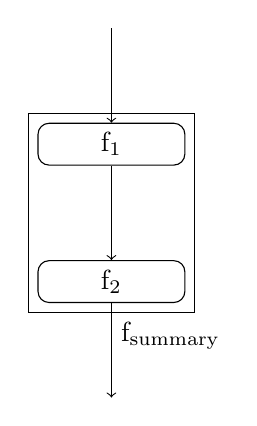
\begin{tikzpicture}[->,
            node distance = 12mm,
            start chain = going below,
            box/.style = {draw,rounded corners,fill=white,
                on chain,align=center,inner xsep=8mm},
            unbox/.style = {on chain,align=center},
            edge/.style = {midway}]
            \coordinate[on chain] (begin);
            \node[box](b1) {f\textsubscript{1}};
            \node[box](b2) {f\textsubscript{2}};
            \coordinate[on chain] (end);
            \node[draw,fit=(b1) (b2)](summary) {};
            \node[below right] at (summary.south) {f\textsubscript{summary}};
            \path[]
                (begin) edge (b1)
                (b1) edge (b2)
                (b2) edge (end);
        \end{tikzpicture}
    }}
    \subfloat[\label{fig:m121:fig1:b}] {{
        \tt
        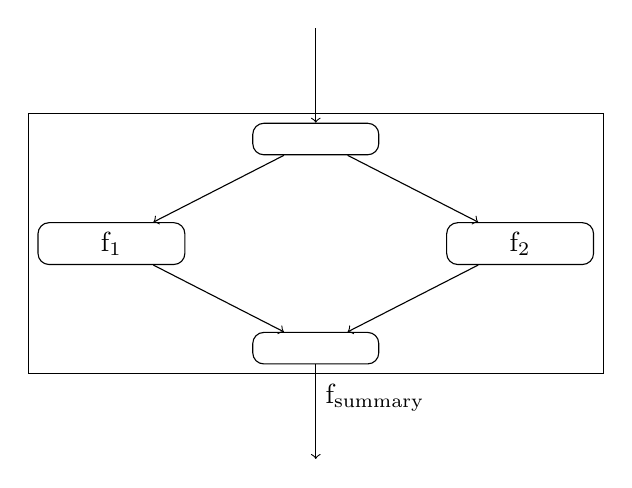
\begin{tikzpicture}[->,
            node distance = 12mm,
            start chain = going below,
            box/.style = {draw,rounded corners,fill=white,
                on chain,align=center,inner xsep=8mm},
            unbox/.style = {on chain,align=center},
            edge/.style = {midway}]
            \coordinate[on chain] (begin);
            \node[box, inner ysep=2mm](b1) {};
            \node[box, below left=of b1](b2) {f\textsubscript{1}};
            \node[box, below right=of b1](b3) {f\textsubscript{2}};
            \node[box, below=of b1, below left=of b3, inner ysep=2mm](b4) {};
            \coordinate[on chain] (end) {};
            \path[]
                (begin) edge (b1)
                (b1) edge (b2)
                (b1) edge (b3)
                (b2) edge (b4)
                (b3) edge (b4)
                (b4) edge (end);
            \node[draw, fit=(b1)(b2)(b3)(b4)](summary) {};
            \node[below right] at (summary.south) {f\textsubscript{summary}};
        \end{tikzpicture}
    }}
    \subfloat[\label{fig:m121:fig1:c}] {{
        \tt
        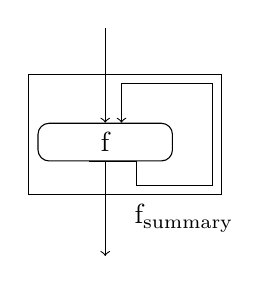
\begin{tikzpicture}[->,
            node distance = 12mm,
            start chain = going below,
            box/.style = {draw,rounded corners,fill=white,
                on chain,align=center,inner xsep=8mm},
            unbox/.style = {on chain,align=center},
            edge/.style = {midway}]
            \coordinate[on chain] (begin);
            \node[box](b1) {f};
            \coordinate[on chain] (end) {};
            \path[]
                (begin) edge (b1)
                (b1) edge (end);
            \draw (b1.230) -| coordinate (l1) ++ (0.6,-0.3) -| coordinate (l2) ([xshift=5mm]b1.east) |-
            coordinate (l3) ([yshift=5mm]b1.50) -- coordinate (l4) (b1.50);
            \node[draw, fit=(b1) (l1) (l2) (l3) (l4)](summary) {};
            \node[below right] at (summary.south) {f\textsubscript{summary}};
        \end{tikzpicture}
    }}
    \caption{}


\end{figure}

\begin{itemize}
    \item The summary functions for larger regions are based on the transfer
    functions of the smaller sub-regions.
    \item The summary functions may involve sophisticated symbolic analysis.
    \item The fallback summary transfer functions can be described using
    composition, meet, and closure operators on transfer functions (for 
    reducible graphs).

    The loops can be captures by the structure that there is a loop body and a
    back edge, the value for it is being captured by the closure. Closure
    means to repeat f one or more times, potentially unbounded.
    \item More sophisticated summary transfer functions can often be described
    using composition, meet, and closure operations on transfer functions.
\end{itemize}

\subsection{Transfer Function Operations}

\begin{figure}[H]
    \centering
    \subfloat[\centering Composition \label{fig:m121:fig2:a}] {{
        \tt
        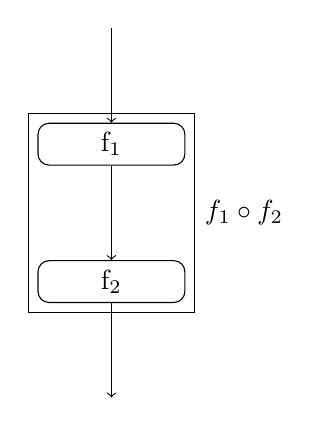
\begin{tikzpicture}[->,
            node distance = 12mm,
            start chain = going below,
            box/.style = {draw,rounded corners,fill=white,
                on chain,align=center,inner xsep=8mm},
            unbox/.style = {on chain,align=center},
            edge/.style = {midway}]
            \coordinate[on chain] (begin);
            \node[box](b1) {f\textsubscript{1}};
            \node[box](b2) {f\textsubscript{2}};
            \coordinate[on chain] (end);
            \node[draw,fit=(b1) (b2)](summary) {};
            \node[right] at (summary.east) {$f_1 \circ f_2$};
            \path[]
                (begin) edge (b1)
                (b1) edge (b2)
                (b2) edge (end);
        \end{tikzpicture}
    }}
    \subfloat[\centering Meet\label{fig:m121:fig2:b}] {{
        \tt
        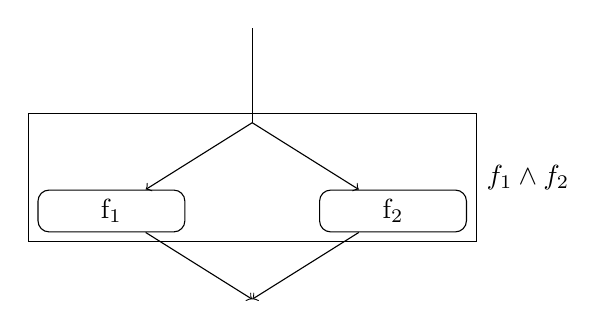
\begin{tikzpicture}[->,
            node distance = 12mm,
            start chain = going below,
            box/.style = {draw,rounded corners,fill=white,
                on chain,align=center,inner xsep=8mm},
            unbox/.style = {on chain,align=center},
            edge/.style = {midway}]
            \coordinate[on chain] (begin);
            \coordinate[on chain] (dummy);
            \node[box, below left=of dummy](b2) {f\textsubscript{1}};
            \node[box, below right=of dummy](b3) {f\textsubscript{2}};
            \coordinate[on chain, below=of dummy, below left=of b3] (end) {};
            \path[]
                (begin) edge[-] (dummy)
                (dummy) edge (b2)
                (dummy) edge (b3)
                (b2) edge (end)
                (b3) edge (end);
            \node[draw, fit=(dummy)(b2)(b3)](summary) {};
            \node[right] at (summary.east) {$f_1 \wedge f_2$};
        \end{tikzpicture}
    }}
    \subfloat[\centering Closure\label{fig:m121:fig2:c}] {{
        \tt
        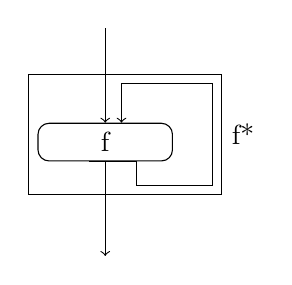
\begin{tikzpicture}[->,
            node distance = 12mm,
            start chain = going below,
            box/.style = {draw,rounded corners,fill=white,
                on chain,align=center,inner xsep=8mm},
            unbox/.style = {on chain,align=center},
            edge/.style = {midway}]
            \coordinate[on chain] (begin);
            \node[box](b1) {f};
            \coordinate[on chain] (end) {};
            \path[]
                (begin) edge (b1)
                (b1) edge (end);
            \draw (b1.230) -| coordinate (l1) ++ (0.6,-0.3) -| coordinate (l2) ([xshift=5mm]b1.east) |-
            coordinate (l3) ([yshift=5mm]b1.50) -- coordinate (l4) (b1.50);
            \node[draw, fit=(b1) (l1) (l2) (l3) (l4)](summary) {};
            \node[right] at (summary.east) {f*};
        \end{tikzpicture}
    }}
    \caption{}


\end{figure}

\subsubsection{Example: Constant Propagation}

\begin{minipage}{0.4\textwidth}
    \tt
    \captionsetup{type=figure}
    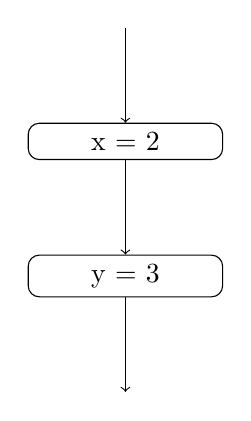
\begin{tikzpicture}[->,
        node distance = 12mm,
        start chain = going below,
        box/.style = {draw,rounded corners,fill=white,
            on chain,align=center,inner xsep=8mm},
        unbox/.style = {on chain,align=center},
        edge/.style = {midway}]
        \coordinate[on chain] (begin);
        \node[box](b1) {x = 2};
        \node[box](b2) {y = 3};
        \coordinate[on chain] (end);
        \path[]
            (begin) edge (b1)
            (b1) edge (b2)
            (b2) edge (end);
    \end{tikzpicture}
    \captionof{figure}{Constant Propagation: Composition}
    \label{fig:m121:const_prop_composition}
\end{minipage}
\hfill
\begin{minipage}{0.5\textwidth}
    \begin{lstlisting}
f1(in) {
    in $\cup$ {(x:2)}
}
f2(in) {
    in $\cup$ {(y:3)}
}
f1 $\circ$ f2(in) {
    in $\cup$ {(x:2), (y:3)}
}
    \end{lstlisting}
\end{minipage}

\begin{minipage}{0.4\textwidth}
    \tt
    \captionsetup[]{type=figure}
    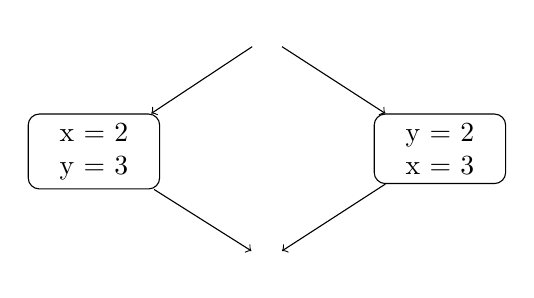
\begin{tikzpicture}[->,
        node distance = 12mm,
        start chain = going below,
        box/.style = {draw,rounded corners,fill=white,
            on chain,align=center, inner xsep=4 mm},
        unbox/.style = {on chain,align=center},
        edge/.style = {midway}]
        \node[on chain, inner xsep=5mm] (begin) {~};
        \node[box, below left=of begin](b2) {x = 2 \\ y = 3};
        \node[box, below right=of begin](b3) {y = 2 \\ x = 3};
        \node[on chain, below=of begin, below left=of b3, inner xsep=5mm] (end) {~};
        \path[]
            (begin) edge (b2)
            (begin) edge (b3)
            (b2) edge (end)
            (b3) edge (end);
    \end{tikzpicture}
    \captionof{figure}{Constant Propagation: Meet}
    \label{fig:m121:const_prop_meet}
\end{minipage}
\hfill
\begin{minipage}{0.5\textwidth}
  \begin{lstlisting}
f1(in) {
    in $\cup$ {(x,2), (y,3)}
}
f2(in) {
    in $\cup$ {(y,2), (x,3)}
}
f1 $\wedge$ f2 (in) {
    f1(in) $\wedge$ f2(in)
}
  \end{lstlisting}  
\end{minipage}

\subsubsection{Example: Available Expressions}

\begin{minipage}{0.4\textwidth}
    \tt
    \captionsetup{type=figure}
    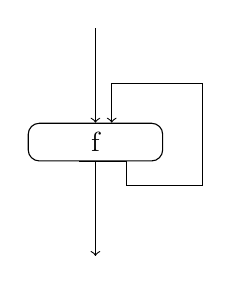
\begin{tikzpicture}[->,
        node distance = 12mm,
        start chain = going below,
        box/.style = {draw,rounded corners,fill=white,
            on chain,align=center,inner xsep=8mm},
        unbox/.style = {on chain,align=center},
        edge/.style = {midway}]
        \coordinate[on chain] (begin);
        \node[box](b1) {f};
        \coordinate[on chain] (end) {};
        \path[]
            (begin) edge (b1)
            (b1) edge (end);
        \draw (b1.230) -| coordinate (l1) ++ (0.6,-0.3) -| coordinate (l2) ([xshift=5mm]b1.east) |-
        coordinate (l3) ([yshift=5mm]b1.50) -- coordinate (l4) (b1.50);
    \end{tikzpicture}
    \captionof{figure}{Available Expressions}

    \begin{lstlisting}
while x != n:
    x = x + 1
    \end{lstlisting}
\end{minipage}
\hfill
\begin{minipage}{0.5\textwidth}
    \begin{lstlisting}
f(in) {
    if in[x] != n
        in{x $\leftarrow$ in[x] + 1} 
            // Updation on in
    else
        in
}
    \end{lstlisting}

    Fallback Closure:
    \begin{lstlisting}
f* (in) {
    in {x $\leftarrow \bot$}
}
    \end{lstlisting}

    Symbolic Closure:
    \begin{lstlisting}
f* (in) {
    in {x $\leftarrow$ max(in(x), n)}
}
    \end{lstlisting}
\end{minipage}

\subsection{Composing GEN/KILL Transfers}

Consider the example of reaching definitions.
\begin{lstlisting}
f1(in) = gen1 $\cup$ (in - kill1)
f2(in) = gen2 $\cup$ (in - kill2)

f1 $\circ$ f2(in) = gen2 $\cup$ ((gen1 $\cup$ (in - kill1)) - kill2)
f1 $\wedge$ f2(in) = gen1 $\cup$ (in - kill1) $\cup$ gen2 $\cup$ (in - kill2)
f1* (in) = gen1 $\cup$ (in - kill2)
\end{lstlisting}

For closure, notice that \texttt{f1(f1(x)) = f1(x)}

%\include{../module122}
%\include{../module123} 
%\include{../module124}
%\include{../module125} 
%\include{../module126}
%\include{../module127} 
%\include{../module128}
%\include{../module129} 
%\include{../module130}
%\include{../module131} 
%\include{../module132}
%\include{../module133} 
%\include{../module134}
%\include{../module135} 
%\include{../module136}
%\include{../module137} 
%\include{../module138}
%\include{../module139} 
%\include{../module140}
%\include{../module141} 
%\include{../module142}
%\include{../module143} 
%\include{../module144}
%\include{../module145} 
%\include{../module146}
%\include{../module147} 
%\include{../module148}
%\include{../module149} 
%\include{../module150}
\end{document}
